\section{Metodología}

\subsection{Materiales y herramientas previstos}
La consigna establece el uso de una Spartan Edge Accelerator Board
con FPGA Spartan-7 XC7S15, el shield multifunción UTEC, cable USB-C
y programador JTAG HS2. El entorno de referencia es Vivado 2025.1;
EDA Playground se admite como alternativa para la simulación
funcional~\cite{guialab2}. La versión y el equipamiento efectivamente
utilizados se registrarán al desarrollar las pruebas.

\subsection{Especificación de la interfaz}
Ambas partes conservan la entidad \texttt{alu}. El bus de doce bits
\texttt{SW} contiene los operandos y el opcode, según la
Tabla~\ref{tab:interfaz}. Las salidas son \texttt{Result}, de cuatro
bits, y las banderas \texttt{Carry} y \texttt{Zero}, de un bit cada
una. La señal \texttt{AR\_3V3\_EN} debe mantenerse en
\texttt{'0'} y asignarse al pin L13 para habilitar los 3,3 V de los
dip-switches; el estándar de E/S indicado es
\texttt{LVCMOS33}~\cite{guialab2}.

La Figura~\ref{fig:alu_parte_a} presenta la vista general de la
Parte A: separación del bus de entrada, bloque combinacional de
la ALU y conexiones con los LEDs y la habilitación del shield.

\begin{figure*}[!t]
\centering
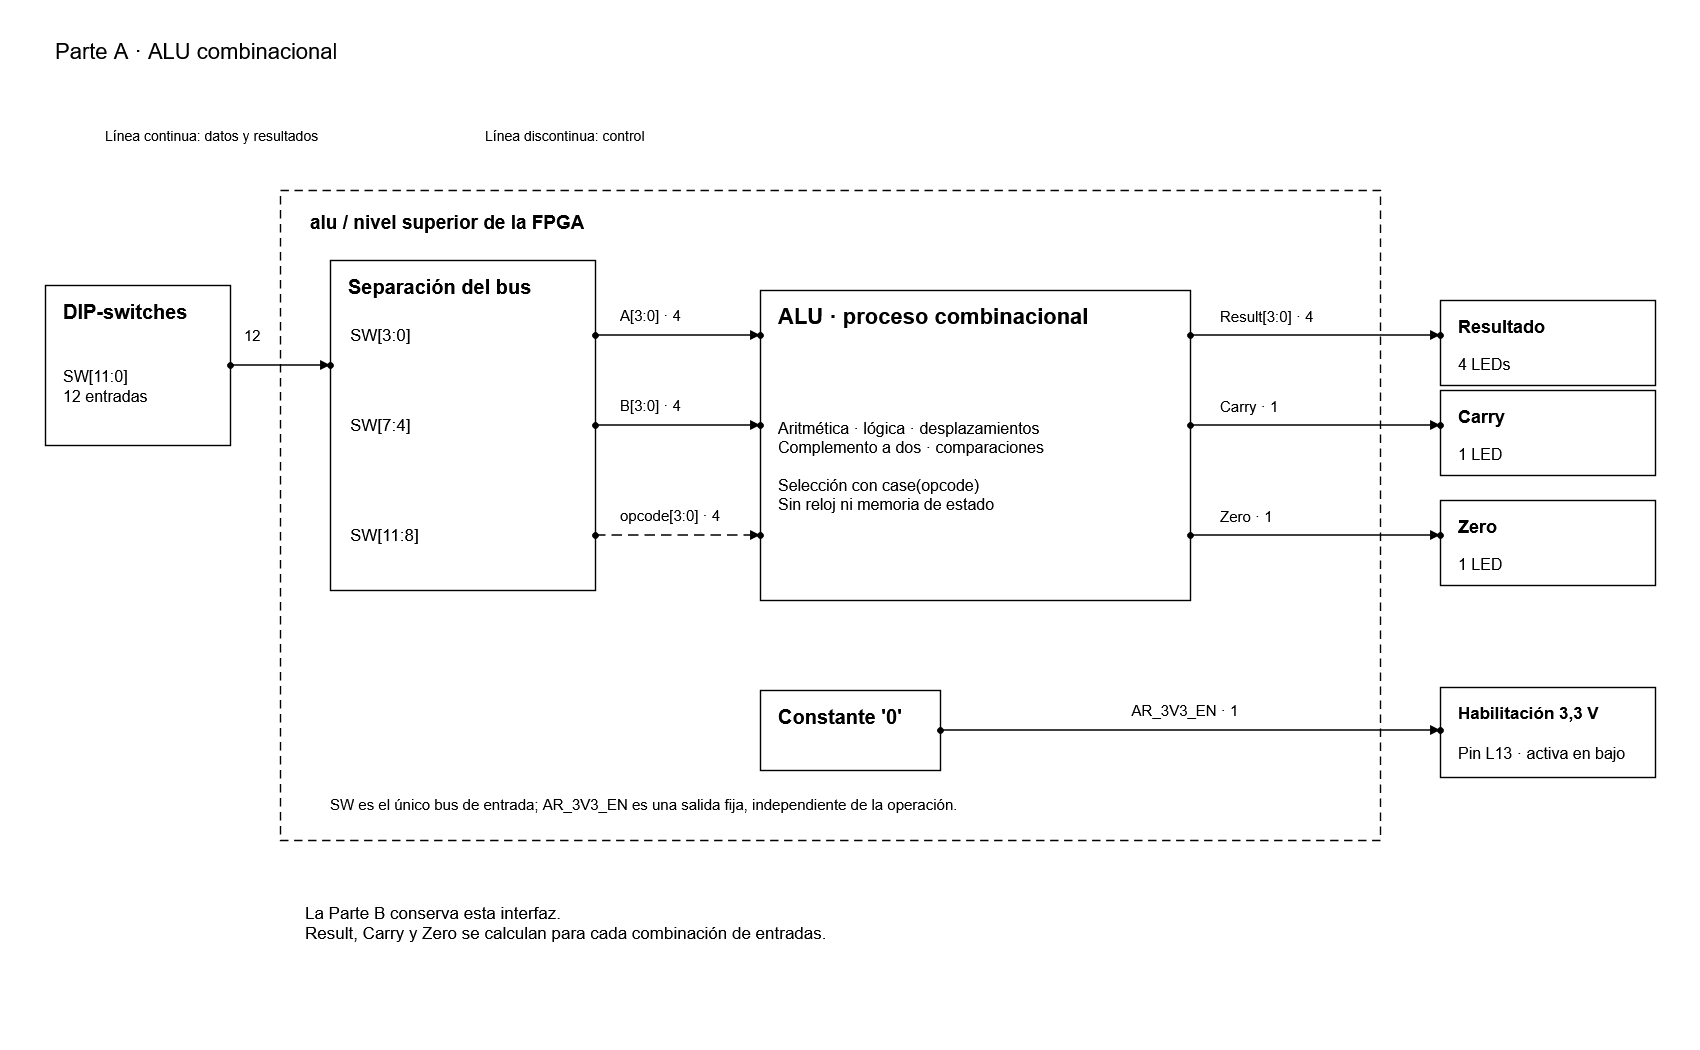
\includegraphics[width=\textwidth]{imagenes/alu_parte_a.png}
\caption{Vista general de la ALU monolítica y su interfaz con el shield UTEC (Parte A).}
\label{fig:alu_parte_a}
\end{figure*}

\begin{table}[htbp]
\centering
\caption{Organización del bus de entrada}
\label{tab:interfaz}
\begin{tabular}{lll}
\toprule
Campo & Bits de \texttt{SW} & Ancho\\
\midrule
$A$ & \texttt{3 downto 0} & 4 bits\\
$B$ & \texttt{7 downto 4} & 4 bits\\
Opcode & \texttt{11 downto 8} & 4 bits\\
\bottomrule
\end{tabular}
\end{table}

\subsection{Operaciones requeridas}
La Tabla~\ref{tab:operaciones} reproduce las operaciones definidas
en la consigna~\cite{guialab2}. Los desplazamientos son lógicos,
de una posición, y las comparaciones devuelven \texttt{0001}
cuando la condición se cumple y \texttt{0000} en caso contrario.

\begin{table}[htbp]
\centering
\caption{Operaciones de la ALU}
\label{tab:operaciones}
\small
\begin{tabular}{cll}
\toprule
Opcode & Operación & Función\\
\midrule
\texttt{0000} & $A+B$ & Suma\\
\texttt{0001} & $A-B$ & Resta\\
\texttt{0010} & $A\mathbin{\mathrm{AND}}B$ & AND bit a bit\\
\texttt{0011} & $A\mathbin{\mathrm{OR}}B$ & OR bit a bit\\
\texttt{0100} & $A\mathbin{\mathrm{XOR}}B$ & XOR bit a bit\\
\texttt{0101} & $\mathrm{NOT}\ A$ & Inversión de bits\\
\texttt{0110} & $A\ll1$ & Desplazamiento izquierdo\\
\texttt{0111} & $A\gg1$ & Desplazamiento derecho\\
\texttt{1000} & $A+1$ & Incremento de $A$\\
\texttt{1001} & $A-1$ & Decremento de $A$\\
\texttt{1010} & $B+1$ & Incremento de $B$\\
\texttt{1011} & $B-1$ & Decremento de $B$\\
\texttt{1100} & $\mathrm{comp2}(A)$ & Complemento a dos de $A$\\
\texttt{1101} & $\mathrm{comp2}(B)$ & Complemento a dos de $B$\\
\texttt{1110} & $A=B$ & Comparación de igualdad\\
\texttt{1111} & $A>B$ & Comparación de magnitud\\
\bottomrule
\end{tabular}
\end{table}

\subsection{Organización del desarrollo}
En la Parte A se describió la ALU en \texttt{alu.vhd}, mediante un
único proceso combinacional sensible a $A$, $B$ y opcode, con
selección mediante \texttt{case}. Se asignaron valores por defecto
a las variables temporales y se calculó Zero a partir del resultado
de la operación. La segunda etapa prevé reorganizar el sistema en \texttt{adder4},
\texttt{arith\_unit}, \texttt{logic\_unit}, \texttt{shift\_unit}
y \texttt{compare\_unit}, conectados desde un nivel superior
estructural. La unidad aritmética utilizará una sola instancia
del sumador. Se prevé verificar los bloques por separado y después
reutilizar los estímulos de la Parte A para contrastar la ALU completa.

La Figura~\ref{fig:alu_parte_b} muestra la arquitectura propuesta
para la Parte B. Los módulos aritmético, lógico, de desplazamiento
y de comparación producen resultados intermedios; la selección
controlada por opcode determina el resultado final y Carry.
Zero se calcula a partir del resultado seleccionado.

Para verificar la Parte A se implementó \texttt{tb\_alu.vhd}, que
recorre los dieciséis opcodes y los dieciséis valores posibles de
cada operando. Cada estímulo se mantiene durante 10 ns antes de
comparar las salidas con un modelo de referencia basado en enteros.
Las comprobaciones con \texttt{assert} abarcan Result, Carry, Zero
y la salida fija de habilitación del shield. Este intervalo organiza
la simulación funcional; no representa una medición de retardo del
circuito físico.

\begin{figure*}[!t]
\centering
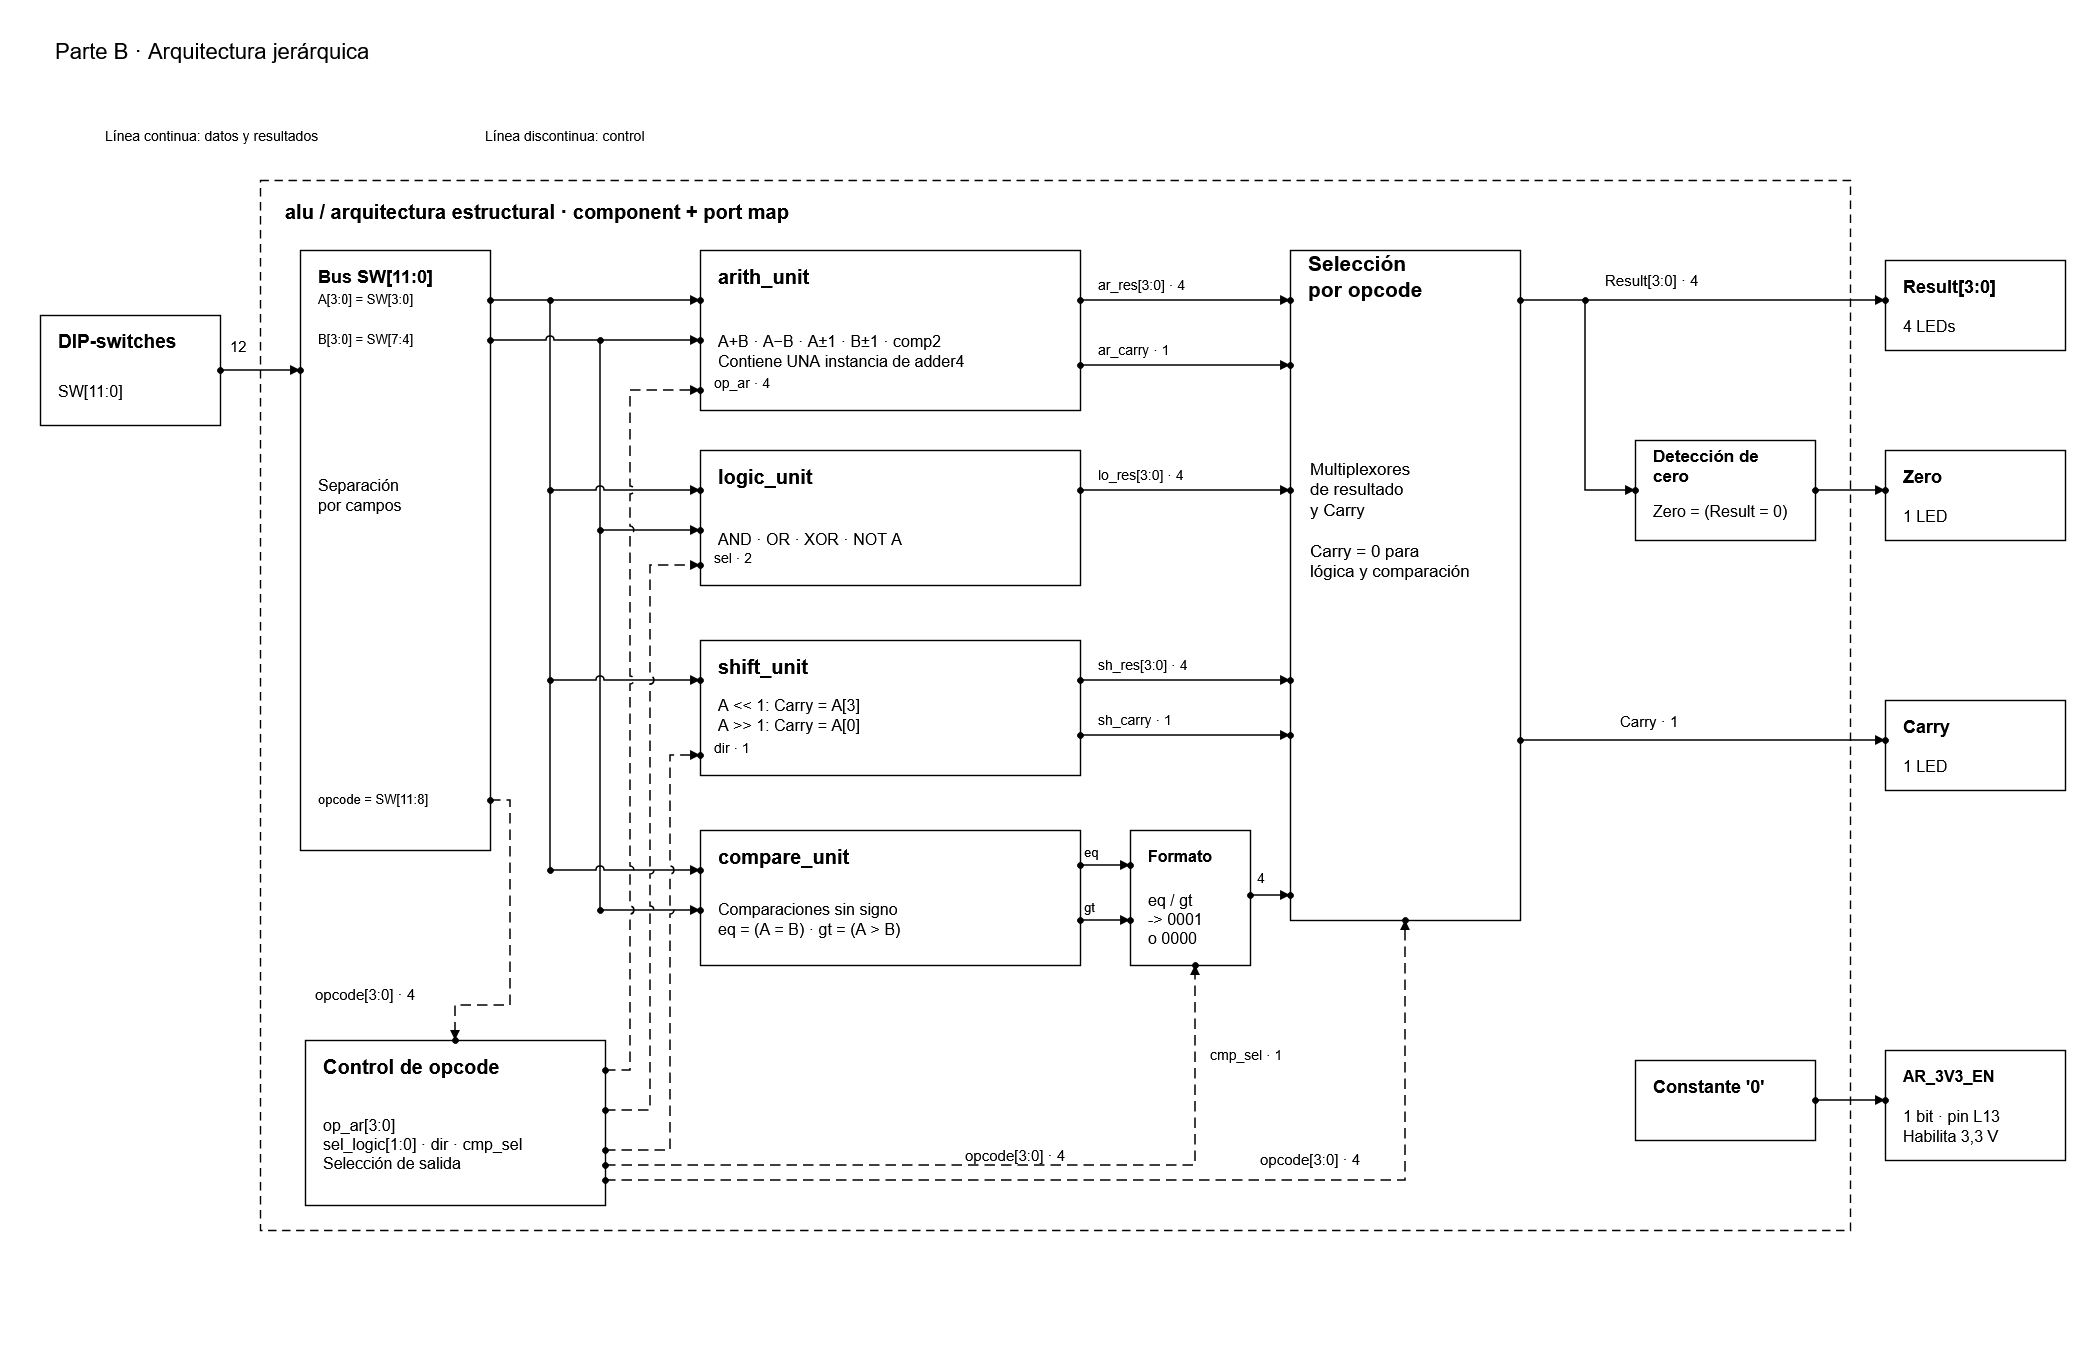
\includegraphics[width=\textwidth]{imagenes/alu_parte_b.png}
\caption{Arquitectura jerárquica de la Parte B: módulos, buses de datos, señales de control y selección de las salidas.}
\label{fig:alu_parte_b}
\end{figure*}

\subsection{Selección de operandos del sumador}
La Tabla~\ref{tab:operandos} define cómo obtener las ocho operaciones
aritméticas con un único sumador de cuatro bits. Las señales $x$ e
$y$ son los operandos seleccionados que se conectan a sus entradas
$a$ y $b$; \texttt{cin} aporta el acarreo de entrada. Los vectores
constantes y los operandos tienen cuatro bits, y la inversión se
realiza bit a bit. En todos los casos, el resultado corresponde a
los cuatro bits de salida $s$, mientras que \texttt{cout} se adapta
según la convención de banderas de la sección siguiente.

La Figura~\ref{fig:unidad_aritmetica} detalla la unidad aritmética:
la selección de operandos y la adaptación de la bandera rodean a
una única instancia de \texttt{adder4}. La tabla de selección
expresa las conexiones requeridas para cada operación, sin agregar
sumadores independientes.

\begin{figure*}[!t]
\centering
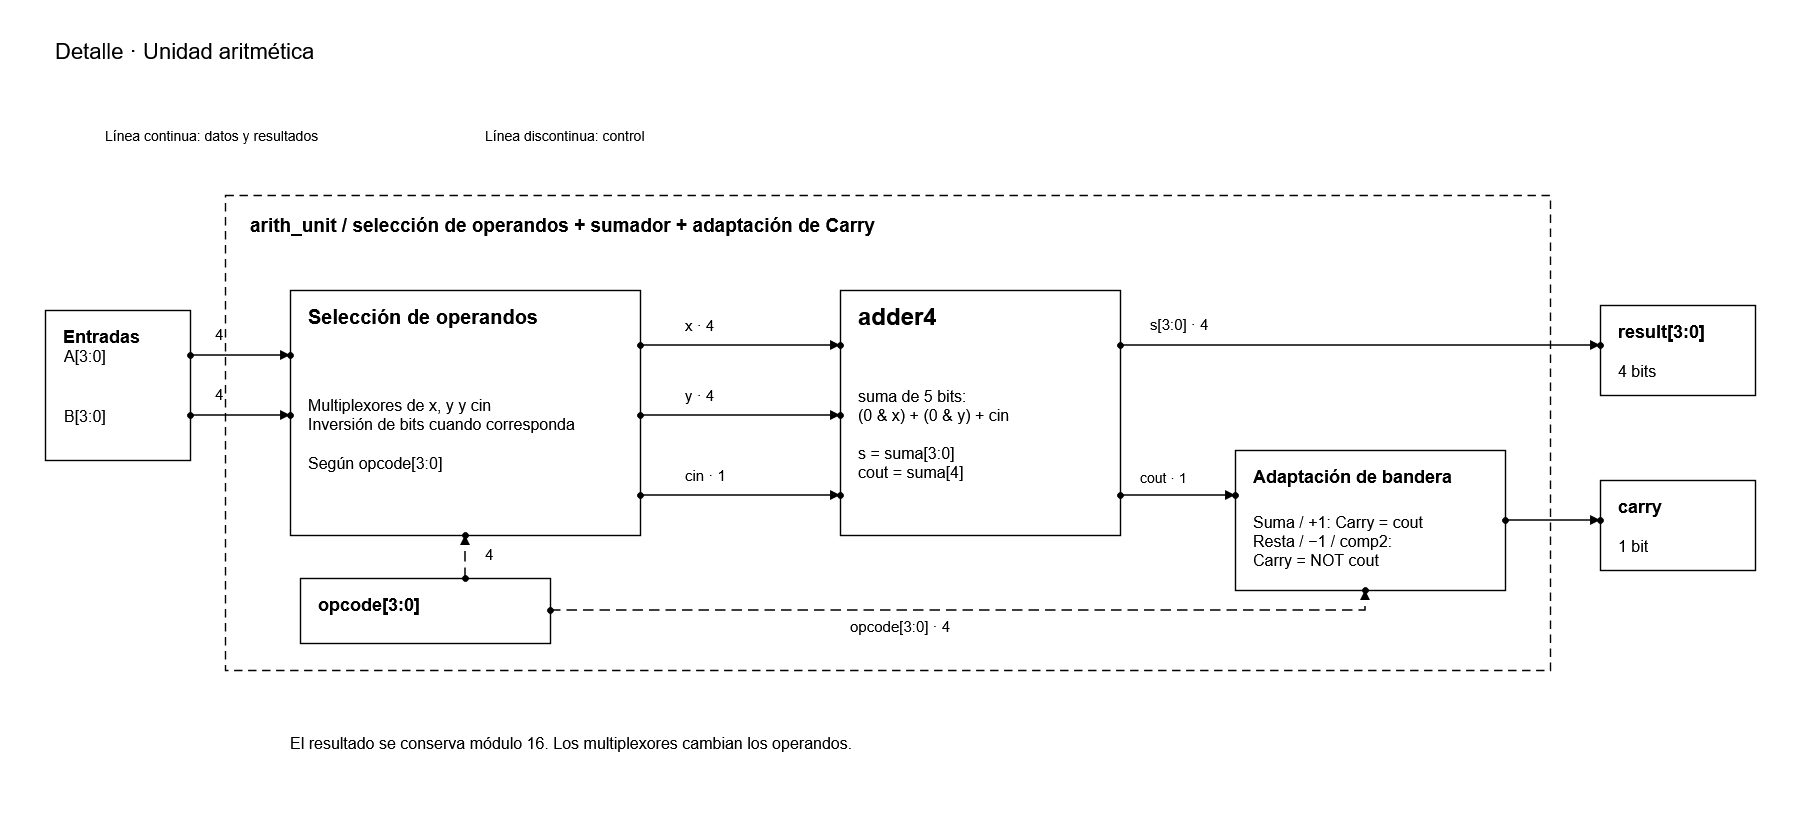
\includegraphics[width=\textwidth]{imagenes/unidad_aritmetica.png}
\caption{Detalle de la unidad aritmética de la Parte B: selección de operandos, sumador reutilizado y adaptación de Carry.}
\label{fig:unidad_aritmetica}
\end{figure*}

\begin{table}[htbp]
\centering
\caption{Selección de entradas del sumador reutilizado}
\label{tab:operandos}
\small
\setlength{\tabcolsep}{4pt}
\begin{tabular}{clcccc}
\toprule
Opcode & Operación & $x$ & $y$ & \texttt{cin} & Resultado\\
\midrule
\texttt{0000} & $A+B$ & $A$ & $B$ & 0 & $s(3:0)$\\
\texttt{0001} & $A-B$ & $A$ & $\overline{B}$ & 1 & $s(3:0)$\\
\texttt{1000} & $A+1$ & $A$ & \texttt{0000} & 1 & $s(3:0)$\\
\texttt{1001} & $A-1$ & $A$ & \texttt{1111} & 0 & $s(3:0)$\\
\texttt{1010} & $B+1$ & $B$ & \texttt{0000} & 1 & $s(3:0)$\\
\texttt{1011} & $B-1$ & $B$ & \texttt{1111} & 0 & $s(3:0)$\\
\texttt{1100} & $\mathrm{comp2}(A)$ & $\overline{A}$ & \texttt{0000} & 1 & $s(3:0)$\\
\texttt{1101} & $\mathrm{comp2}(B)$ & $\overline{B}$ & \texttt{0000} & 1 & $s(3:0)$\\
\bottomrule
\end{tabular}
\end{table}

\subsection{Convención adoptada para las banderas}
La consigna fija Carry para suma, resta, lógica y comparación,
pero no explicita su significado en las demás operaciones.
Para completar la especificación se adopta la
Tabla~\ref{tab:carry}. Se conserva el criterio de acarreo en
operaciones aditivas y de préstamo en las sustractivas. En la tabla,
$X$ representa el operando $A$ o $B$, según el opcode.

\begin{table}[htbp]
\centering
\caption{Convención adoptada para Carry}
\label{tab:carry}
\small
\begin{tabular}{ll}
\toprule
Operación & Carry vale 1 cuando\\
\midrule
$A+B$ & $A+B\geq16$\\
$A-B$ & $A<B$\\
$X+1$ & $X=15$\\
$X-1$ & $X=0$\\
$\mathrm{comp2}(X)$ & $X\ne0$ (préstamo de $0-X$)\\
Desplazamiento izquierdo & $A(3)=1$ (bit descartado)\\
Desplazamiento derecho & $A(0)=1$ (bit descartado)\\
Lógica y comparación & Nunca; Carry se mantiene en 0\\
\bottomrule
\end{tabular}
\end{table}

El complemento a dos se interpreta como $0-X$, conservando los
cuatro bits del resultado. Por ello, si $X\ne0$ se señala préstamo,
aunque el resultado mostrado sea un vector sin signo. Por ejemplo,
$\mathrm{comp2}(1)=\texttt{1111}$ con Carry en 1, mientras que
$\mathrm{comp2}(0)=\texttt{0000}$ con Carry en 0.

Con la selección de operandos del sumador reutilizado, la adaptación
es Carry igual a \texttt{cout} para suma e incrementos, y Carry
igual a \texttt{not cout} para resta, decrementos y complemento a dos.
Esta regla distingue el acarreo bruto del sumador de la bandera
que se expone en la interfaz.

Los desplazamientos introducen un cero en la posición vacante y
copian a Carry el bit que abandona el vector. Así, desplazar
\texttt{1000} una posición a la izquierda produce \texttt{0000}
con Carry en 1; desplazar \texttt{0001} a la derecha da la misma
combinación de resultado y Carry. Zero vale 1 en ambos ejemplos
porque siempre se calcula sobre los cuatro bits del resultado final,
independientemente de Carry.

Esta convención se aplicará a las Partes A y B y al modelo de
referencia de sus bancos de prueba.
